% ---------------------------------------------------------------------------
% The Bellman circle of value functions
% ECO 629 -- Studies in Quantitative Methods (Stony Brook University)
%
% Build:
%   pdflatex bellman_circle.tex
%   pdftoppm -r 400 -png -singlefile bellman_circle.pdf ../img/bellman_circle
%
% Renders on an opaque white page so the image sits correctly on a white
% card in both the light and the dark theme of the course website.
% ---------------------------------------------------------------------------
\documentclass[border=6pt,11pt]{standalone}

\usepackage[T1]{fontenc}
\usepackage[utf8]{inputenc}
\usepackage[scaled]{helvet}
\renewcommand{\familydefault}{\sfdefault}
\usepackage{amsmath}

\usepackage{xcolor}
\usepackage{tikz}
\usetikzlibrary{arrows.meta,calc}

% ---- house palette --------------------------------------------------------
\definecolor{hsPrimary}{HTML}{2E7EB8}   % borders and arrows
\definecolor{hsFill}{HTML}{EAF1F8}      % light node fill
\definecolor{hsAccent}{HTML}{E0A32E}    % accent, used sparingly
\definecolor{hsText}{HTML}{1F2937}      % body text
\definecolor{hsMuted}{HTML}{5B6B7C}     % subtitles and arrow labels

\pagecolor{white}

% ---- editable labels ------------------------------------------------------
% Node contents: main symbol, name, alternative name
\newcommand{\topSym}{$V(x,\varepsilon)$}
\newcommand{\topName}{(plain) value function}
\newcommand{\topAlt}{}

\newcommand{\rightSym}{$V^\sigma(x), V(x)$}
\newcommand{\rightName}{integrated value function}
\newcommand{\rightAlt}{(ex-ante)}

\newcommand{\bottomSym}{$EV(x,d)$}
\newcommand{\bottomName}{expected value function}
\newcommand{\bottomAlt}{(ex-post)}

\newcommand{\leftSym}{$v(x,d)$}
\newcommand{\leftName}{choice-specific value function}
\newcommand{\leftAlt}{(conditional)}

% Arrow labels, clockwise from the top
\newcommand{\arrTR}{$\displaystyle\int_\Omega \bullet \; q(\varepsilon|x)\,d\varepsilon$}
\newcommand{\arrRB}{$\displaystyle\int_X \bullet \; \pi(x'|x,d)\,dx'$}
\newcommand{\arrBL}{$u(x,d) + \beta\, \bullet$}
\newcommand{\arrLT}{$\displaystyle\max_{d}\,\{\bullet + \varepsilon(d)\}$}

% ---- geometry -------------------------------------------------------------
\newcommand{\R}{3.6}    % radius of the circle the nodes sit on, cm
\newcommand{\gap}{28}   % angular gap left free around each node, degrees

\begin{document}
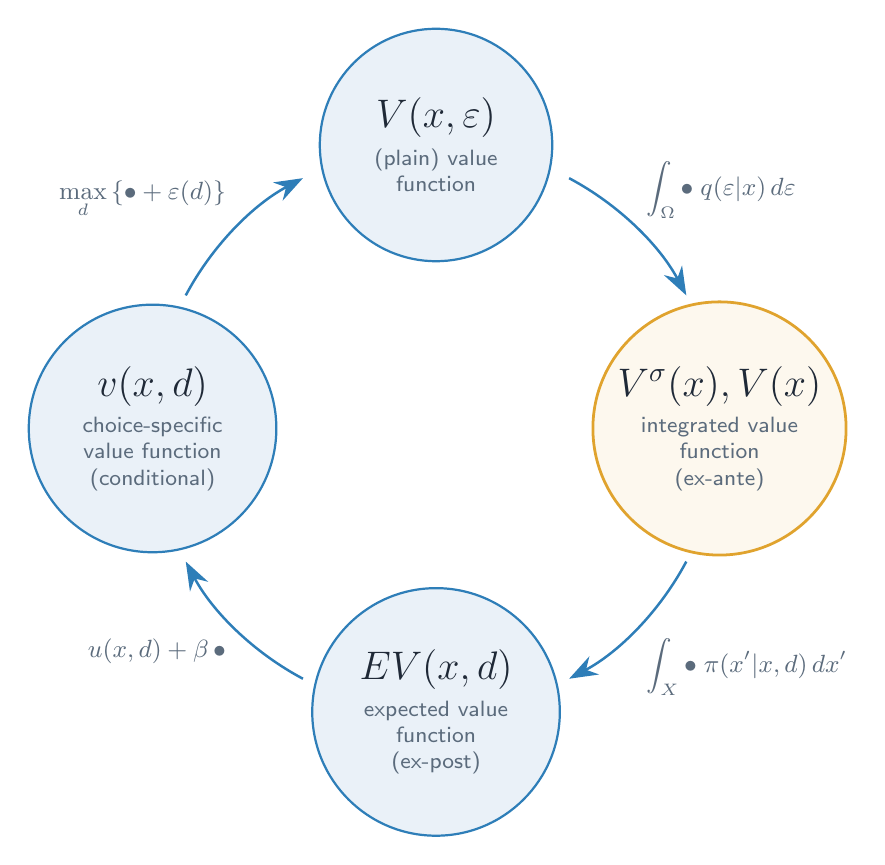
\begin{tikzpicture}[
  font=\sffamily,
  vf/.style={
    circle, draw=hsPrimary, line width=0.8pt, fill=hsFill,
    minimum size=2.9cm, inner sep=2pt, align=center, text=hsText
  },
  vfkey/.style={vf, draw=hsAccent, line width=1pt, fill=hsAccent!8!white},
  flow/.style={
    -{Stealth[length=3.6mm,width=2.6mm]},
    draw=hsPrimary, line width=0.9pt
  },
  lbl/.style={font=\sffamily\small, text=hsMuted}
]

% ---- nodes ----------------------------------------------------------------
\node[vf]    (top)    at (90:\R)  {{\Large\topSym}\\[3pt]
  \parbox{2.5cm}{\centering\footnotesize\color{hsMuted}\topName\\\topAlt}};
\node[vfkey] (right)  at (0:\R)   {{\Large\rightSym}\\[3pt]
  \parbox{2.5cm}{\centering\footnotesize\color{hsMuted}\rightName\\\rightAlt}};
\node[vf]    (bottom) at (-90:\R) {{\Large\bottomSym}\\[3pt]
  \parbox{2.5cm}{\centering\footnotesize\color{hsMuted}\bottomName\\\bottomAlt}};
\node[vf]    (left)   at (180:\R) {{\Large\leftSym}\\[3pt]
  \parbox{2.5cm}{\centering\footnotesize\color{hsMuted}\leftName\\\leftAlt}};

% ---- arrows (clockwise arcs on the same circle) ---------------------------
\draw[flow] (90-\gap:\R)  arc[start angle=90-\gap,  end angle=\gap,      radius=\R];
\node[lbl, anchor=south west] at (45:\R) {\arrTR};
\draw[flow] (-\gap:\R)    arc[start angle=-\gap,    end angle=-90+\gap,  radius=\R];
\node[lbl, anchor=north west] at (-45:\R) {\arrRB};
\draw[flow] (-90-\gap:\R) arc[start angle=-90-\gap, end angle=-180+\gap, radius=\R];
\node[lbl, anchor=north east] at (-135:\R) {\arrBL};
\draw[flow] (180-\gap:\R) arc[start angle=180-\gap, end angle=90+\gap,   radius=\R];
\node[lbl, anchor=south east] at (135:\R) {\arrLT};

\end{tikzpicture}
\end{document}
